\documentclass[11pt,letterpaper]{article}

% Load some basic packages that are useful to have
% and that should be part of any LaTeX installation.
%
% be able to include figures
\usepackage{graphicx}
% get nice colors
\usepackage{xcolor}

% change default font to Palatino (looks nicer!)
\usepackage{apjfonts}
% load some useful math symbols/fonts
\usepackage{latexsym,amsfonts,amsmath,amssymb}

% comfort package to easily set margins
\usepackage[top=1in, bottom=1in, left=1in, right=1in]{geometry}

% control some spacings
%
% spacing after a paragraph
\setlength{\parskip}{.15cm}
% indentation at the top of a new paragraph
\setlength{\parindent}{0.0cm}


\begin{document}

\begin{center}
\Large
{\bf Ay190 -- Worksheet 11} \\
\large
Xiangcheng Ma \\
Date: \today
\end{center}

\section*{Advection Equation}
(1) See the implemented code.

(2) In all the sections, I adopt $\Delta t=0.1$ and $\Delta x=0.1$. First, I take $v=0.9$ and thus $\alpha=0.9<1$. One snapshot at $t=540$ is showed at upper-left panel in Figure \ref{fig1}. In all the plots, numerical solutions are plotted in solid blue lines, analytical solutions are plotted in solid red lines and errors are plotted in solid green lines. For $\alpha=0.9$, the solution is stable.

Then switch $\sigma$ to a value five times smaller than the original one. A snapshot at $t=270$ is plotted in the upper-right panel in Figure \ref{fig1}. The error is highly amplified around the peak.

Finally, change $v$ to 1.5 and thus $\alpha=1.5>1$ and get back to the original $\sigma$ value. A snapshot at $t=78$ is plotted in lower panel in Figure \ref{fig1}. The solution starts to become unstable. The unstability just above $x=0$ may originate from the boundary condition we adopt.

\begin{figure}[bth]
\centering
\begin{tabular}{cc}
    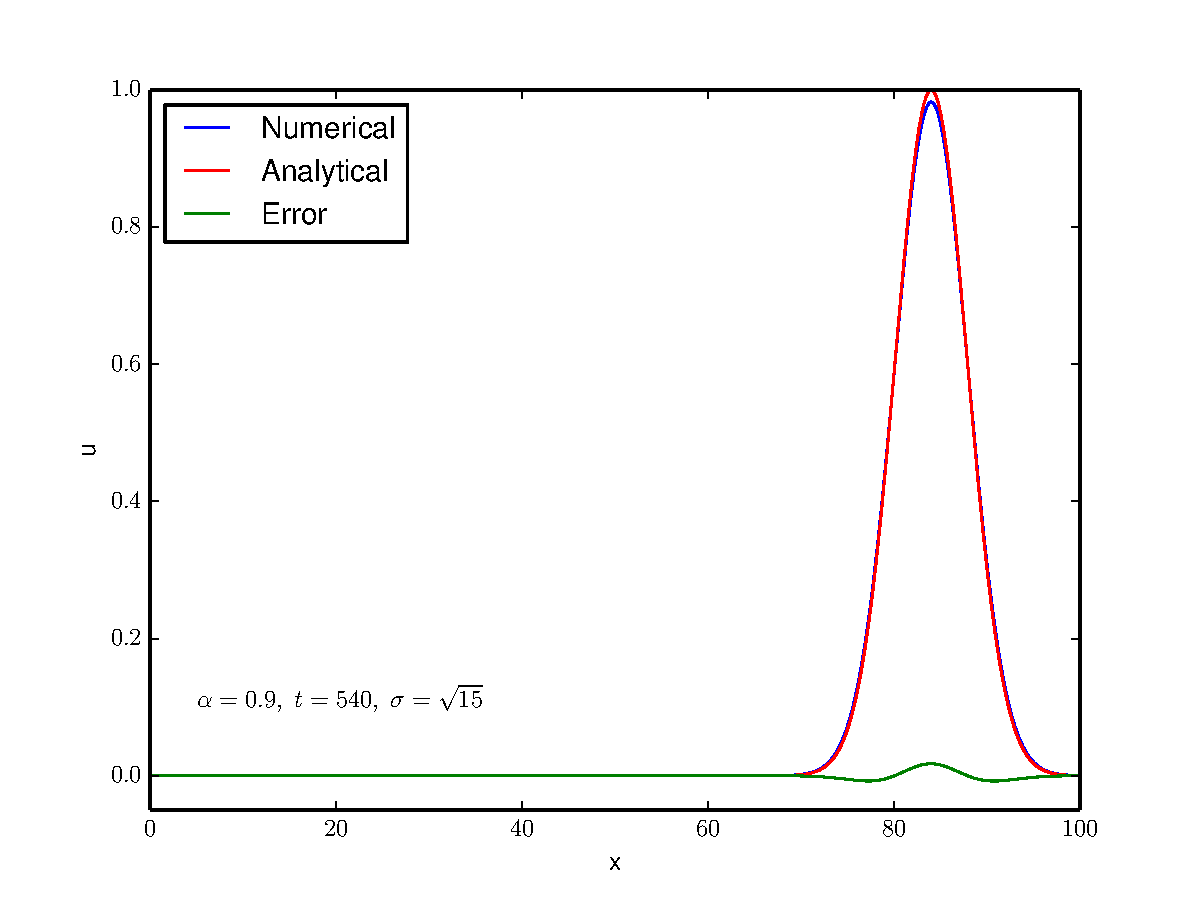
\includegraphics[width={0.49\textwidth}]{fig1.pdf} &
    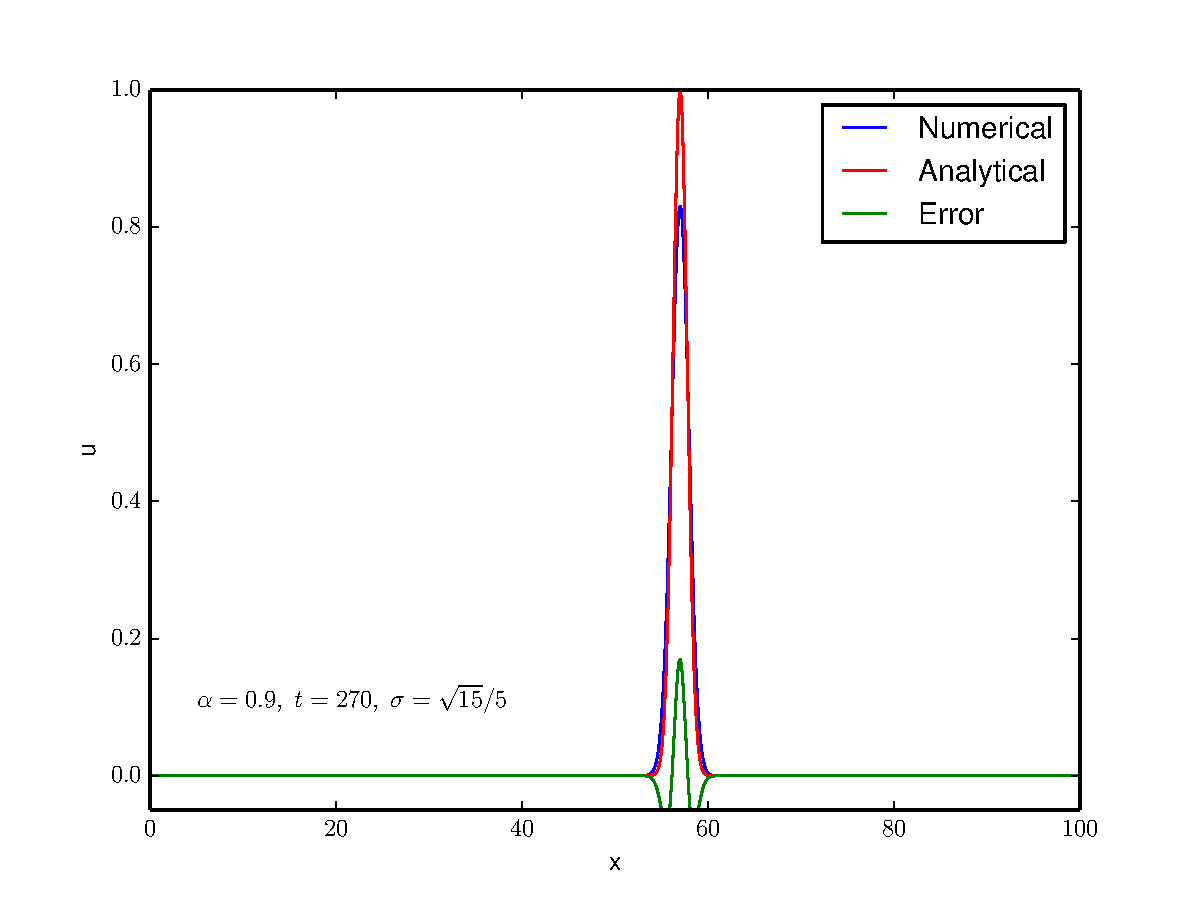
\includegraphics[width={0.49\textwidth}]{fig2.pdf} \\
    \multicolumn{2}{c}{ 
    	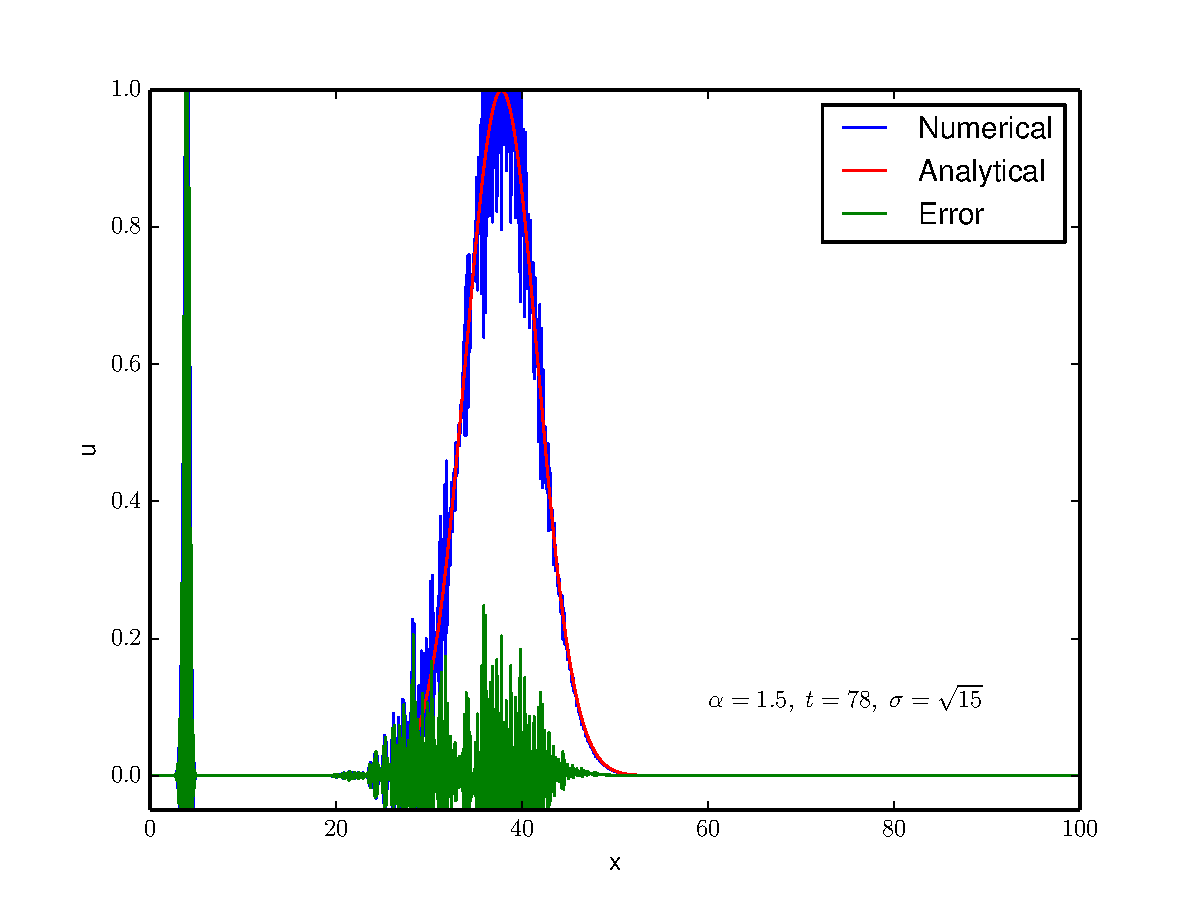
\includegraphics[width={0.49\textwidth}]{fig3.pdf}
    } \\
\end{tabular}
\caption{Upwind method}
\label{fig1}
\end{figure}

(3) In this section, I take $v=0.9$ ($\alpha=0.9$). Two snapshots at $t=90$ and $t=108$ are plotted in Figure \ref{fig2}. We can see that the solution becomes stable at some time between those despite $\alpha<1$.

\begin{figure}[bth]
\centering
\begin{tabular}{cc}
    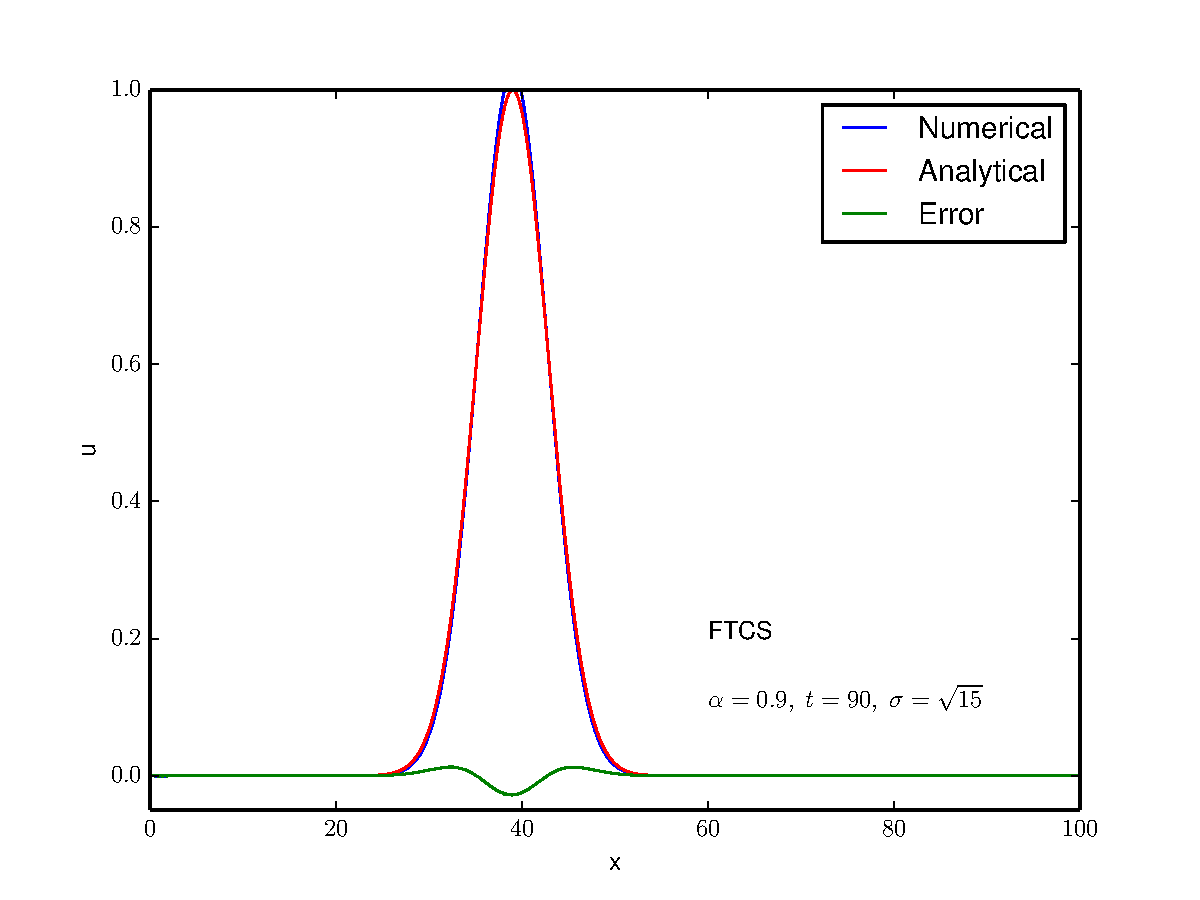
\includegraphics[width={0.49\textwidth}]{fig4.pdf} &
    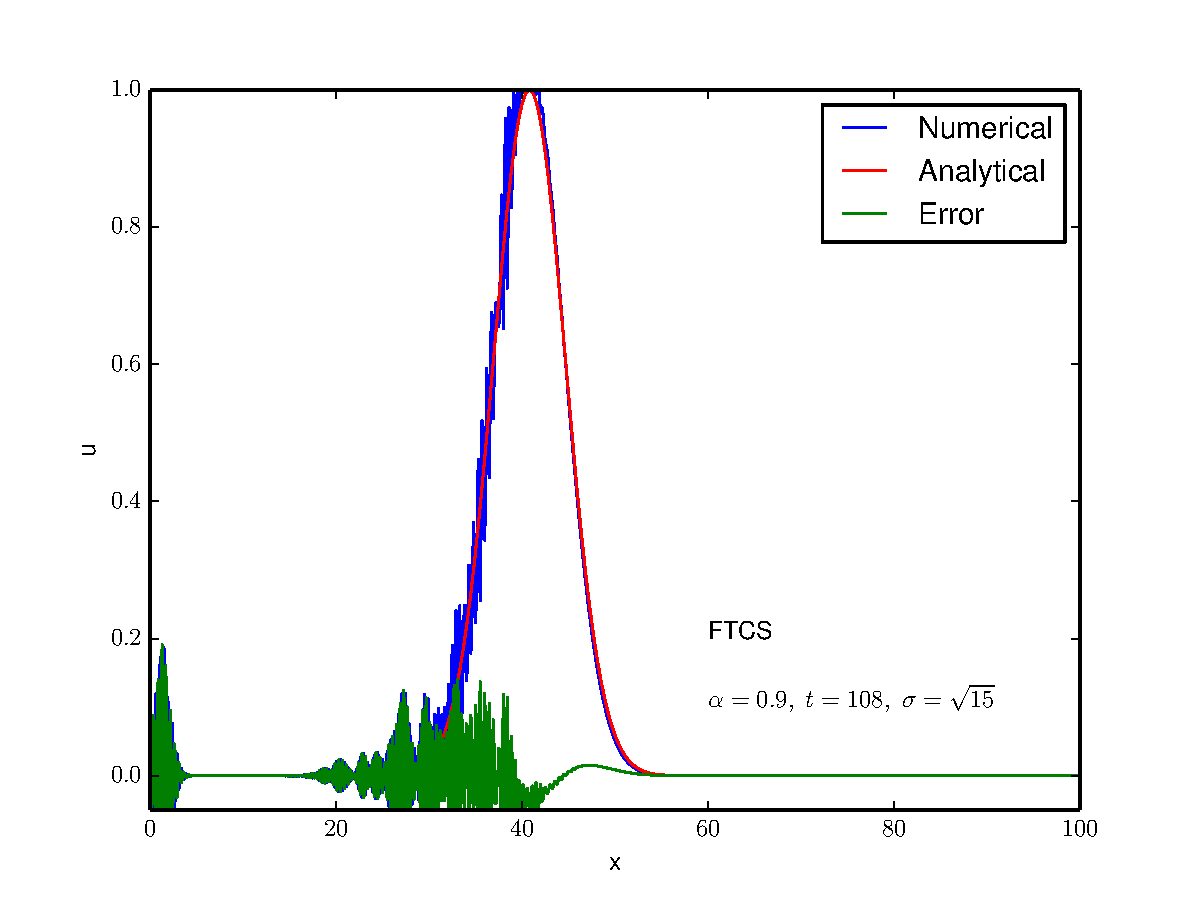
\includegraphics[width={0.49\textwidth}]{fig5.pdf} \\
\end{tabular}
\caption{FTCS method}
\label{fig2}
\end{figure}

(4) I take $v=0.9$ and $v=1.5$, respectively as what I have done in (2). For $\alpha=0.9$, a snapshot at $t=540$ is plotted in Figure \ref{fig3}. For $\alpha=1.5$, two snapshot at $t=78$ and $t=135$ are plotted. The solution is unstable for $\alpha>1$ similar to the upwind case.

\begin{figure}[bth]
\centering
\begin{tabular}{cc}
    \multicolumn{2}{c}{ 
    	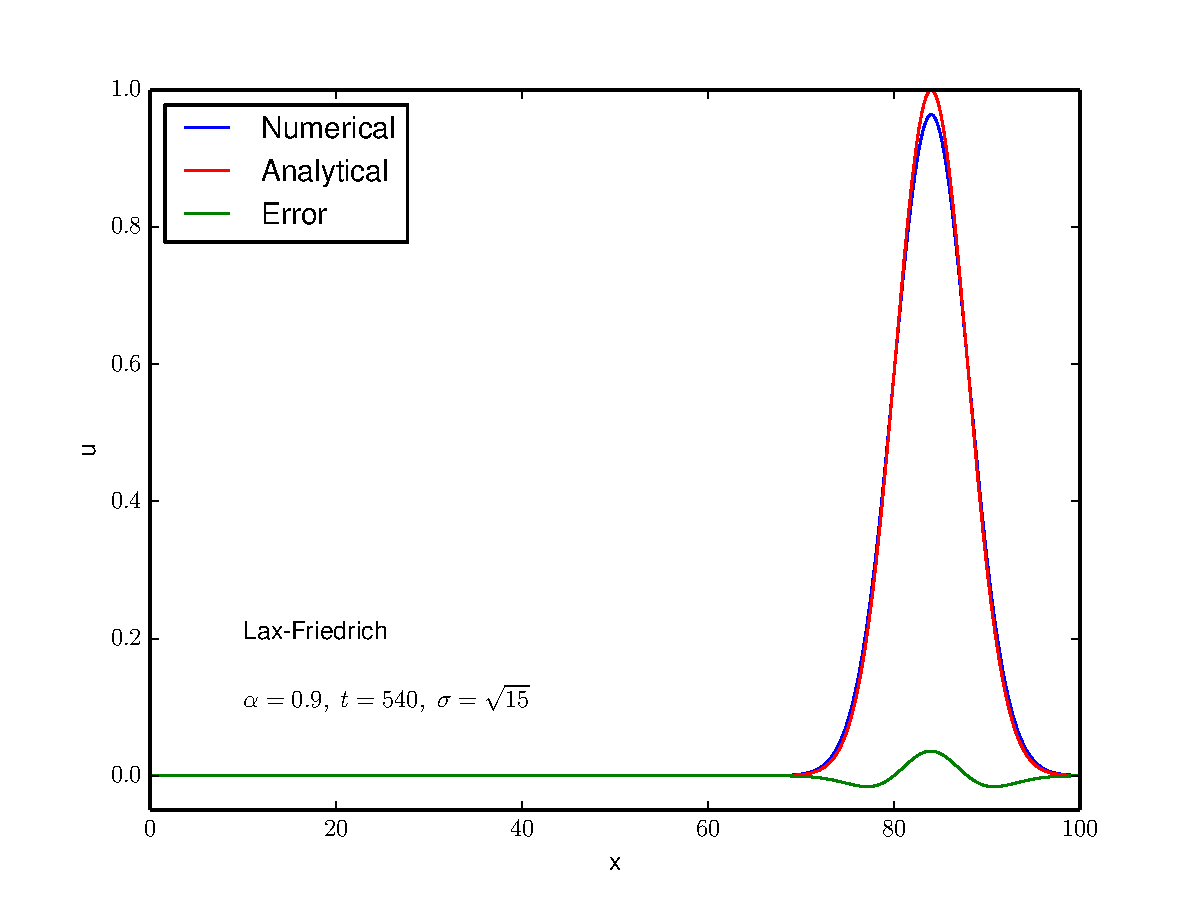
\includegraphics[width={0.49\textwidth}]{fig6.pdf}
    } \\
    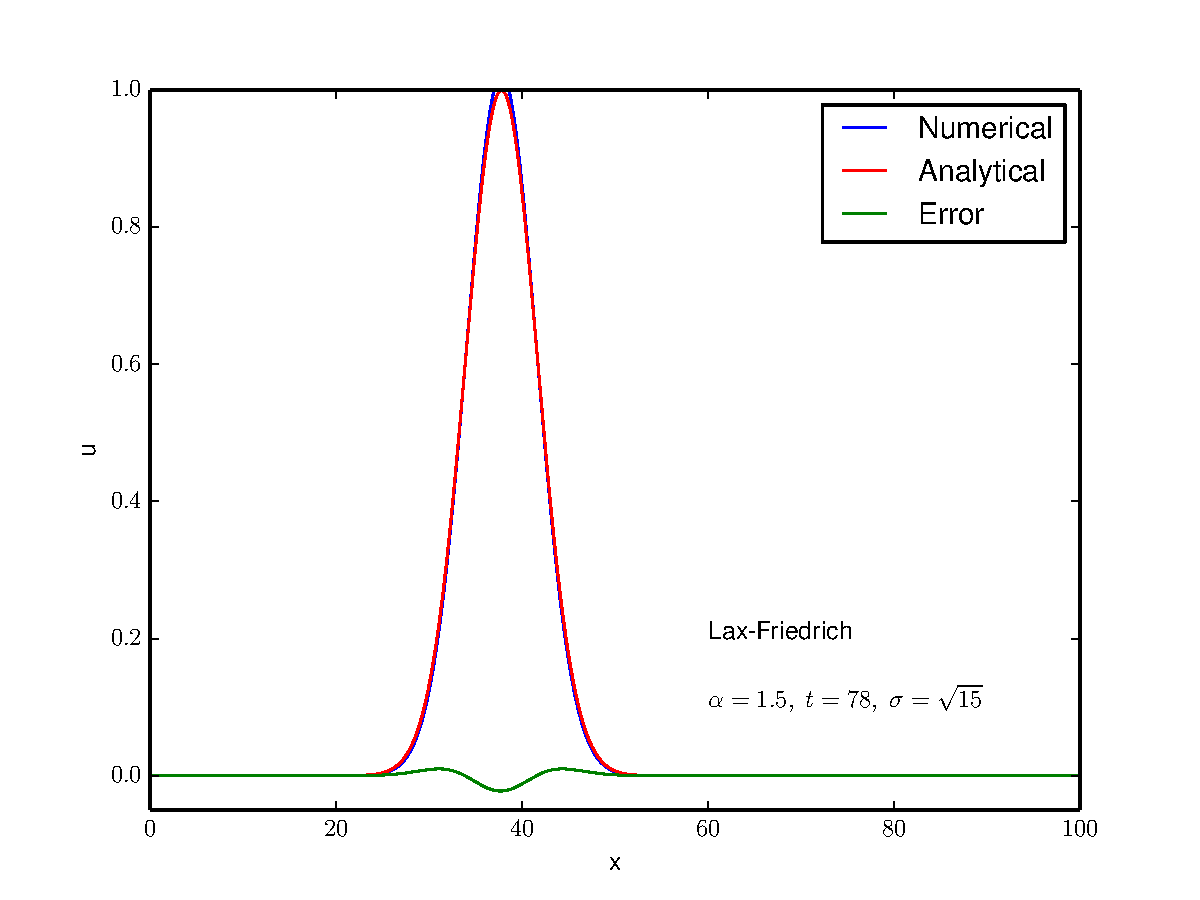
\includegraphics[width={0.49\textwidth}]{fig7.pdf} &
    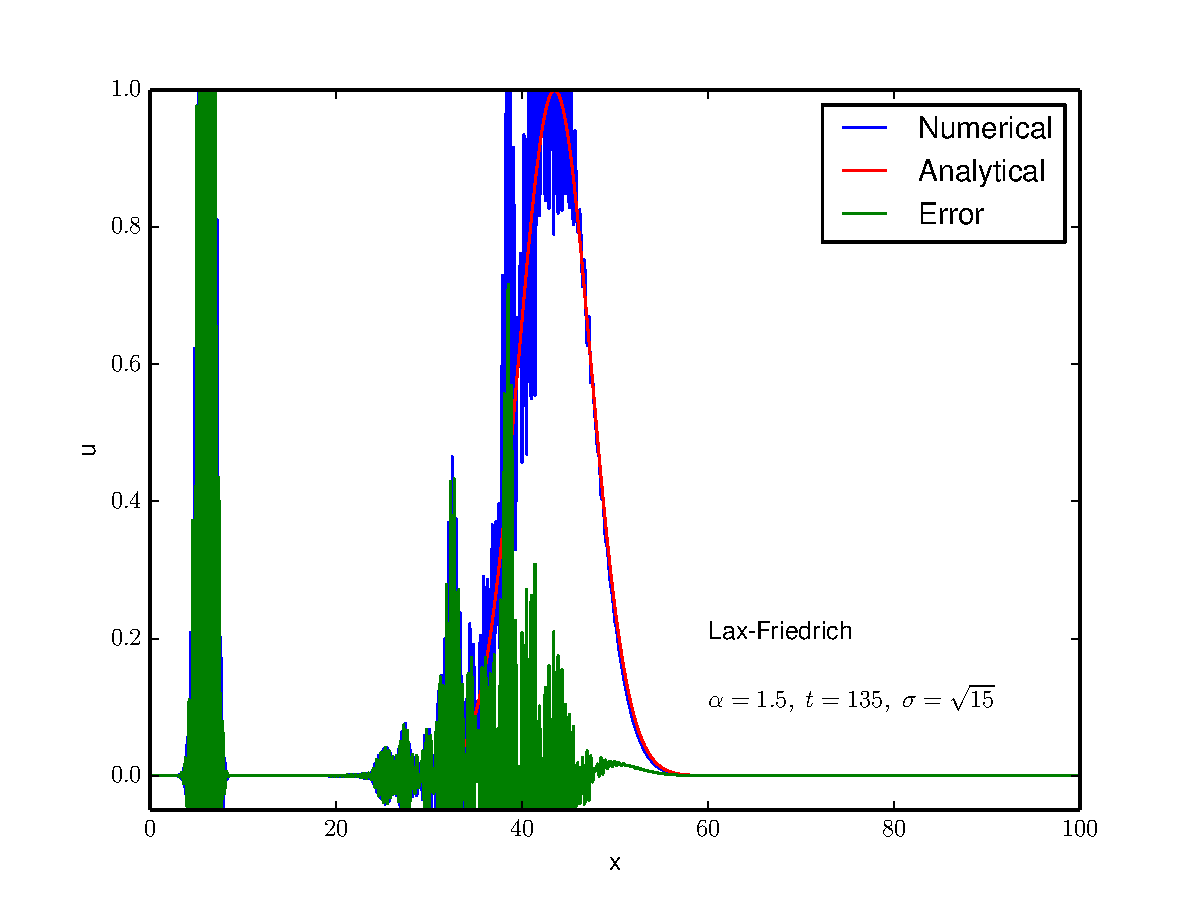
\includegraphics[width={0.49\textwidth}]{fig8.pdf} \\
\end{tabular}
\caption{Lax-Friedrich method}
\label{fig3}
\end{figure}

(5) Three snapshots for Leapfrog method are plotted in Figure \ref{fig4}. This method is unstable for both $\alpha=0.9$ and $\alpha=1.5$.

\begin{figure}[bth]
\centering
\begin{tabular}{cc}
    \multicolumn{2}{c}{ 
    	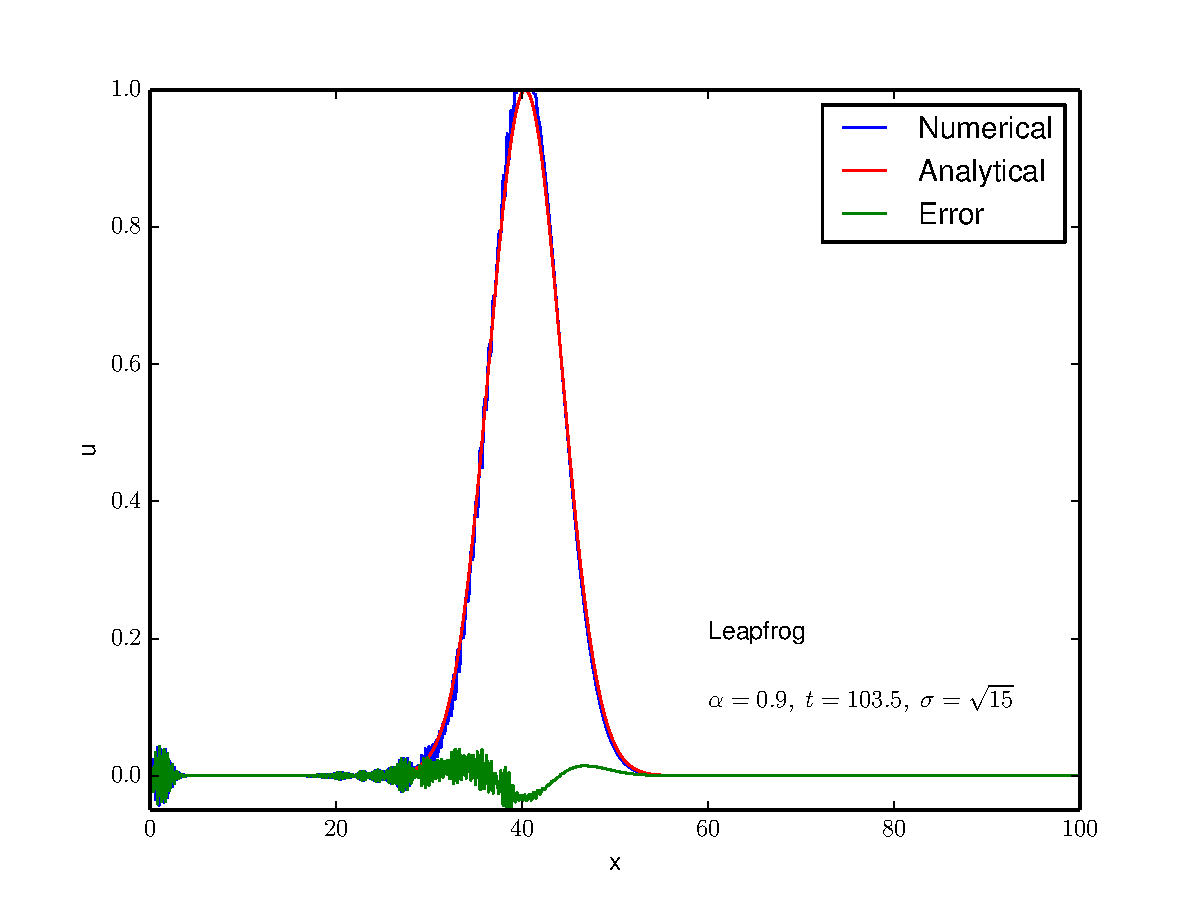
\includegraphics[width={0.49\textwidth}]{fig11.pdf}
    } \\
    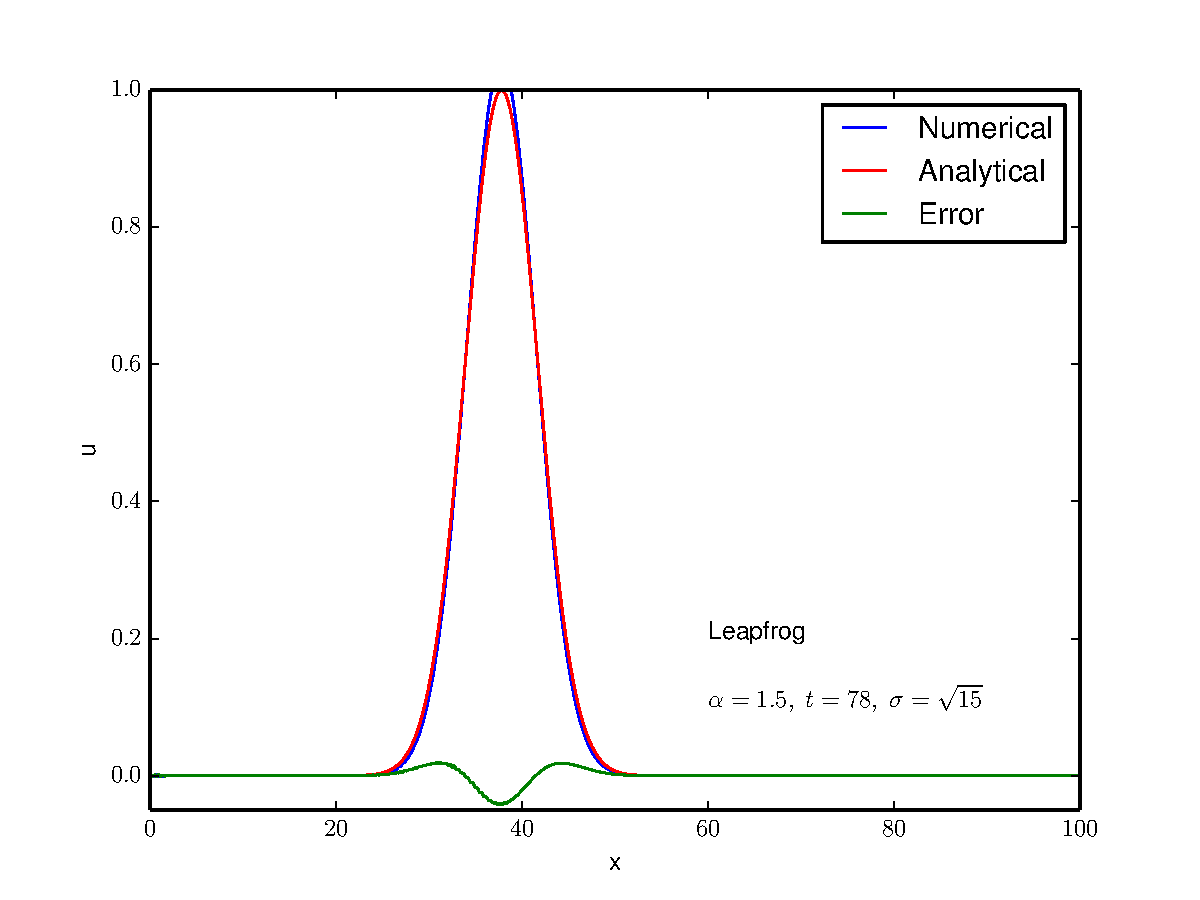
\includegraphics[width={0.49\textwidth}]{fig9.pdf} &
    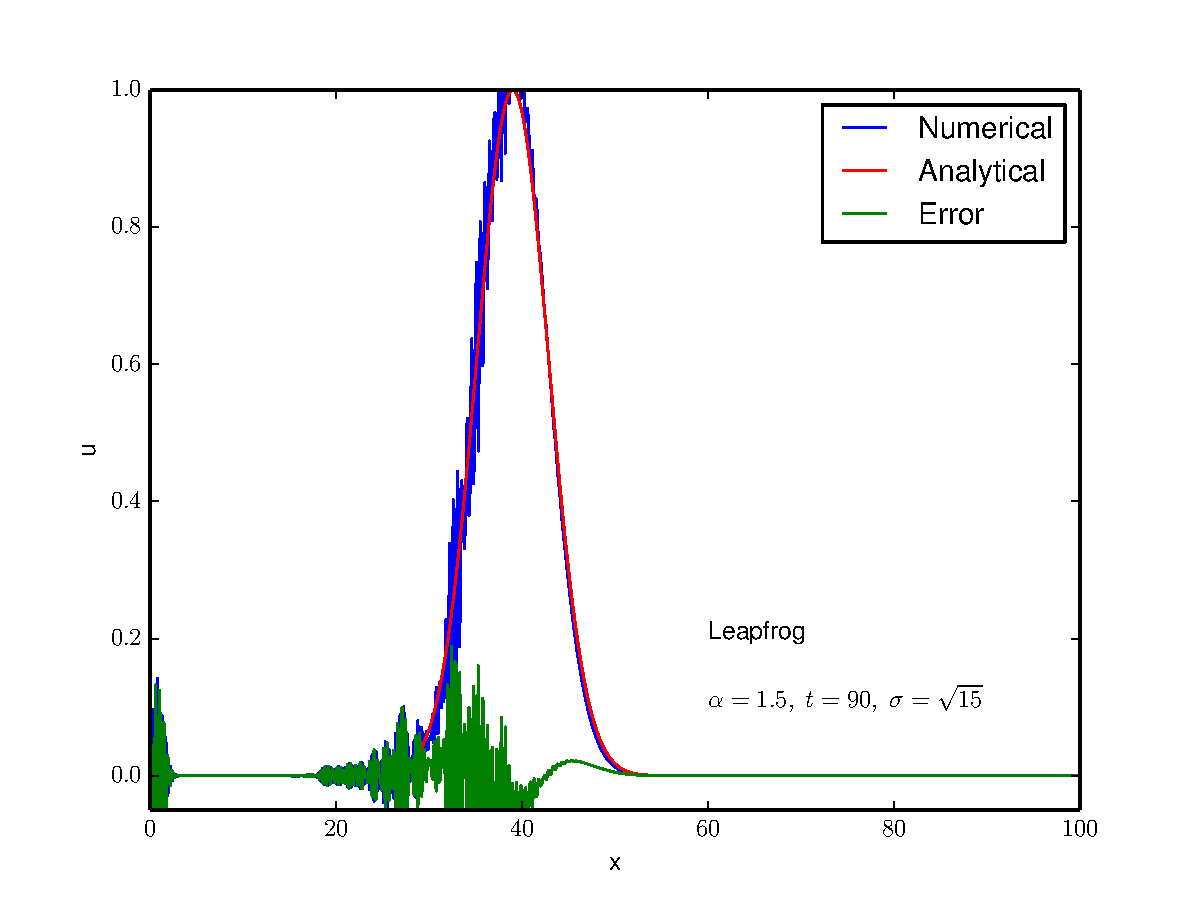
\includegraphics[width={0.49\textwidth}]{fig10.pdf} \\
\end{tabular}
\caption{Leapfrog method}
\label{fig4}
\end{figure}

Two snapshots for $\alpha=0.9$ and $\alpha=1.5$ are plotted in Figure \ref{fig5}. In the former case, the error is much smaller than any other cases. And it seems that the solution becomes unstable much faster than other cases for $\alpha>1$.

\begin{figure}
\centering
\begin{tabular}{cc}
    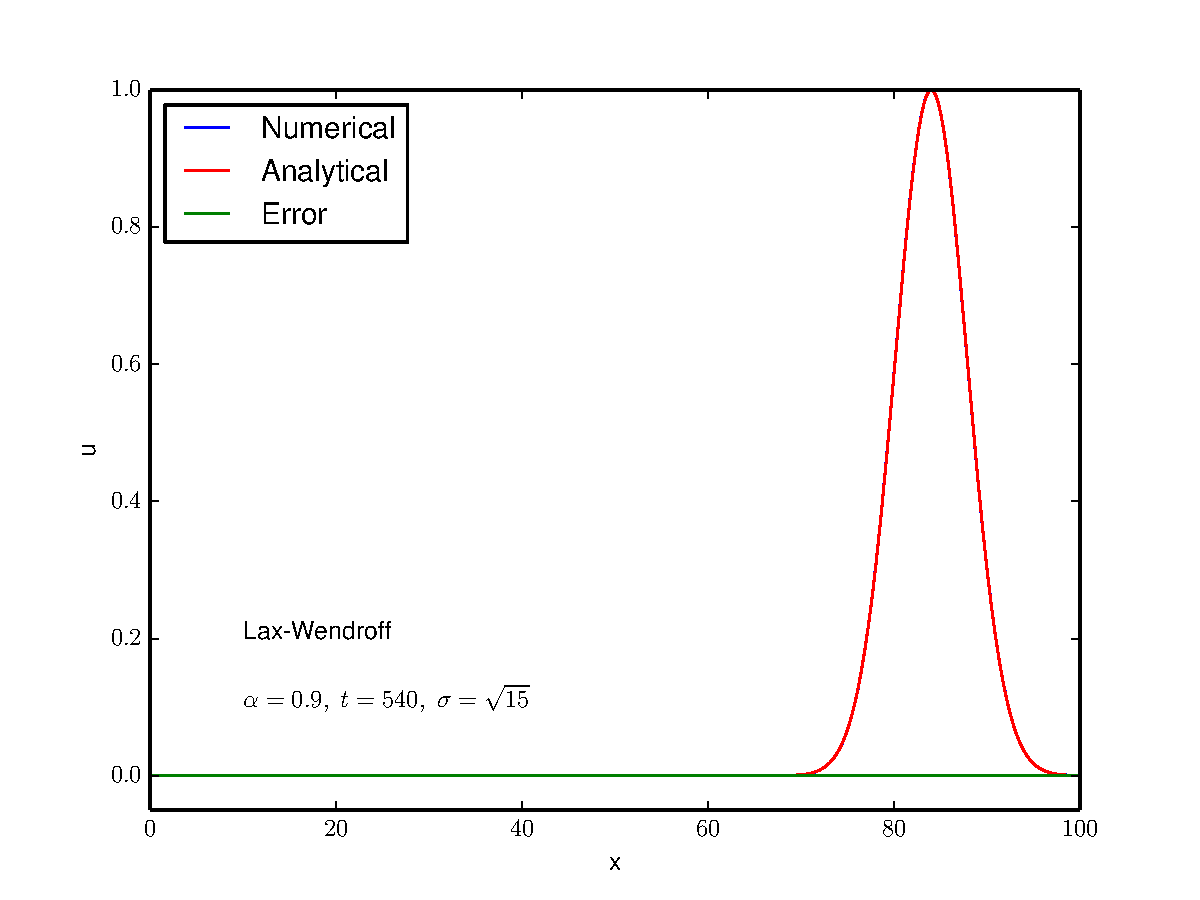
\includegraphics[width={0.49\textwidth}]{fig12.pdf} &
    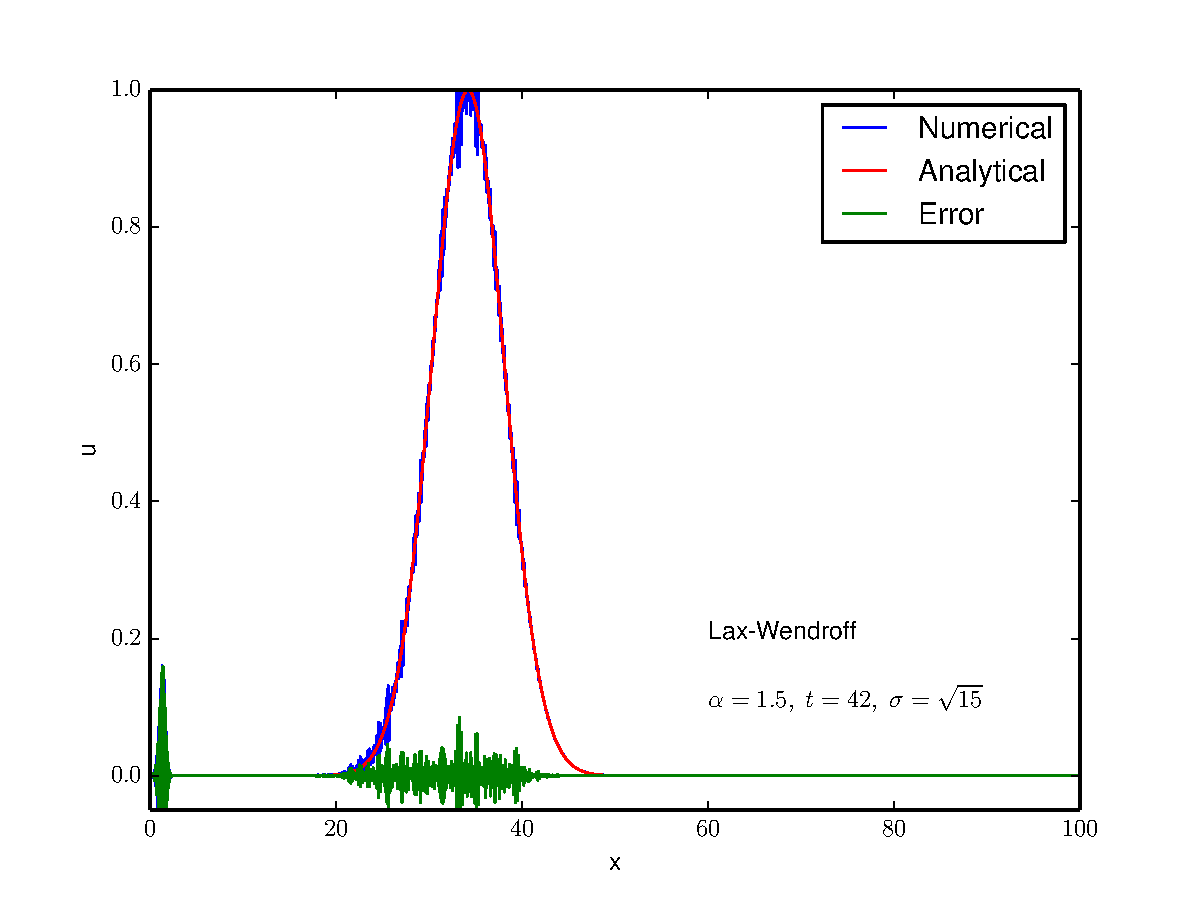
\includegraphics[width={0.49\textwidth}]{fig13.pdf} \\
\end{tabular}
\caption{Lax-Wendroff method}
\label{fig5}
\end{figure}

\end{document}
